\section{Metric Classes}
Conversion of the Workload theory into quantifiable measurements necesitated the creation of workload metric classes. In the interest of finding areas to consolidate actors we left off measuring team workload. Given that cognitive workload describes the difficulties presented by managing resources such as memory and inputs we named that metric class resource. Algorithmic workload anaylzes the difficulties presented by decisions giving rise to the decision metrics.


\begin{figure}
\center
\setlength{\abovecaptionskip}{1mm}
\setlength{\belowcaptionskip}{1mm}
\setlength{\textfloatsep}{1mm}
\setlength{\floatsep}{1mm}
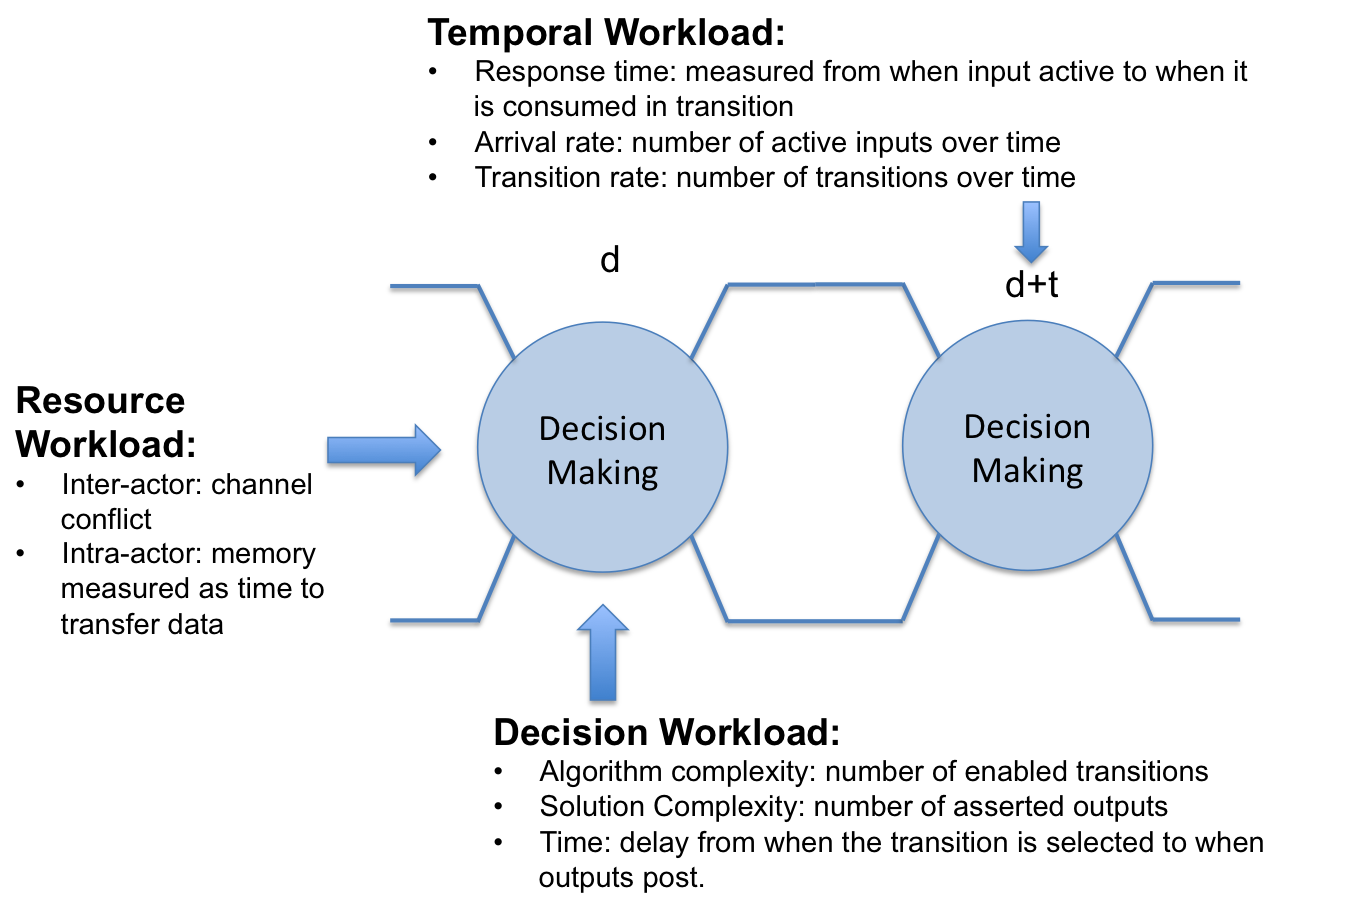
\includegraphics[height=2in]{WorkloadMetrics.png}
\caption{Workload in the model}
\label{fig:WorkloadMetrics}
\end{figure}

\subsection{Resource Metrics}
The model in use lent itself to two distinct ways in to measure Resource Workload. There are a set number of channels connected to each actor and a set amount of data an actor can retain in it's internal memory at a time. Counting the memory accesses and channel inputs viewed in each actor state gives a quantifiable metric for the Research Workload.
Temporal and the model

\subsection{Temporal Metrics}
 There are three different ways the model can measure the temporal workload. The number of transitions that occur over a set period of time gives an accurate reflection of the tempo of a given task. The rate at which inputs activate gives a measurement for the arrival rate of new data while the response time can be calculated by measuring the time it takes for an input to be acted upon after it becomes active.

\subsection{Decision Metrics}
Decision Workload can be broken down into the timing, the complexity of the algorithm, and the complexity of the solution. Timing is calculated by measuring the time when a transition is chosen till the outputs are posted, this gives us a sense of the duration it takes to complete a given task. The algorithm complexity is calculated by counting how many transitions are possible at a given time while the solution complexity measures the number of outputs that are asserted.
